\documentclass[12pt]{article}
\usepackage{setspace}
\usepackage{latexsym}
\usepackage{amssymb,amsmath}
\usepackage[pdftex]{graphics}
\usepackage{graphicx}
\usepackage{amsthm}


\topmargin = -0.5in \textwidth=6.5in \textheight=9in

\oddsidemargin = 0in \evensidemargin = 0in

\DeclareMathSizes{12}{10}{7}{5}
\newcommand{\bphi}{\bar{\phi}}
\newcommand{\bw}{\bar{w}}
\newcommand{\bv}{\bar{v}}
\newcommand{\bF}{\bar{F}}
\newcommand{\bg}{\bar{g}}
\newcommand{\be}{\bar{\eta}}
\newcommand{\br}{\bar{\rho}}
\newcommand{\bmu}{\bar{\mu}}
\newcommand{\bx}{\bar{x}}
\newcommand{\bS}{\bar{S}}
\newcommand{\bT}{\bar{T}}
\newcommand{\sq}{\sqrt{2}}
\newcommand{\hk}{\hat{k}}
\newcommand{\hr}{\hat{r}}
\newcommand{\hy}{\hat{y}}
\newcommand{\hY}{\hat{Y}}
\newcommand{\tx}{\tilde{x}}
\newcommand{\tW}{\tilde{W}}
\newcommand{\tb}{\tilde{b}}
\newcommand{\tg}{\tilde{g}}
\newcommand{\tz}{\tilde{z}}
\newcommand{\eps}{\epsilon}
\newcommand{\teps}{\tilde{\epsilon}}
\newcommand{\tS}{\tilde{S}}
\newcommand{\tA}{\tilde{A}}
\newcommand{\tsigma}{\tilde{\sigma}}
\newcommand{\tlambda}{\tilde{\lambda}}
\newcommand{\ulq}{\underline{q}}
\newcommand{\olq}{\overline{q}}
\newcommand{\ulr}{\underline{r}}
\newcommand{\olr}{\overline{r}}
\newcommand{\Exp}{\ProbOpr{E}}
\newtheorem{theorem}{Theorem}[section]
\newtheorem{corollary}{Corollary}[theorem]
\newtheorem{lemma}[theorem]{Lemma}
\newtheorem{proposition}[theorem]{Proposition}
\input{__macros}
\begin{document}


\title{Low-Precision Random Fourier Features (LP-RFF)}
\author{Avner May, Jian Zhang}
\onehalfspacing
\maketitle

\section{Introduction}
\label{sec:intro}
The goal of this work is to understand whether we can train better kernel approximation models, at lower cost,
by quantizing the random Fourier features [1].  We will analyze, empirically and theoretically, the performance of low-precision random Fourier features (LP-RFF), relative to the full-precision features.  Specifically, we will consider quantizing the features, which take the form $z_i(x) = \sqrt{\frac{2}{m}} \cos(w_i^Tx+b_i)$ into $b$-bits, through some form of quantization scheme (simplest: random rounding). 
When using $b$-bits to represent values in the interval $[-\sqrt{2/m},\sqrt{2/m}]$, we will simply divide this interval evenly into $2^b-1$ sub-intervals.  Letting $\delta = \frac{2\sqrt{2/m}}{2^b-1}$, this allows us to represent the values $\{-\sqrt{2/m},-\sqrt{2/m} + \delta,\ldots,\sqrt{2/m}-\delta, \sqrt{2/m}\}$. \\

\noindent \textbf{Outline}:
\begin{itemize}
	\item Section \ref{sec:kernel_approx}: Analysis of kernel approximation error.
	\item Section \ref{sec:gen}: Analysis of generalization performance.
	\item Section \ref{sec:train}: Training in low-precision.
	\item Section \ref{sec:experiments}: Experiments.
	\item Section \ref{sec:future}: Future Directions.
\end{itemize}

\noindent \textbf{Main questions}:
\begin{itemize}
	\item What can we say about the variance of these low-precision features, in their approximation of the kernel?  Concentration inequalities?
	\item Can we analyze the generalization performance of these features?
	\item Is there an optimal level of precision, with regard to achieving the best kernel approximation performance, or generalization performance, under a fixed memory budget?
	\item How should models be trained on top of these low-precision features? Can we train in low-precision, and if so, what would the effects of such a training scheme be on the performance of the model?
	\item Can we achieve better performance per bit, if we use \textit{variable precision} to store the random Fourier features (by storing directions of highest variance with more bits)?
\end{itemize}

\section{Kernel Approximation Error for LP-RFF}
\label{sec:kernel_approx}

\subsection{Kernel Approximation Variance Analysis}
\noindent\textbf{Definition}:  For $z \in [a,c]$, let $X_z^{a,c}$ be the random variable which with probability $\frac{z-a}{c-a}$ equals $c-z$, and with probability $\frac{c-z}{c-a}$ equals $a-z$.

\begin{lemma}
\label{lemma:qvar}
$\expect{}{X_z^{a,c}} = 0$, and $\var{}{X_z^{a,c}} = (c-z)(z-a) \leq \frac{(c-a)^2}{4}$.
\end{lemma}

\begin{proof}
\begin{eqnarray*}
	\expect{}{X_z^{a,c}} &=&  (c-z)\cdot \frac{z-a}{c-a} + (a-z)\cdot \frac{c-z}{c-a}\\
	&=& 0 .\\
	\var{}{X_z^{a,c}} &=& (c-z)^2\cdot \frac{z-a}{c-a} + (a-z)^2\cdot \frac{c-z}{c-a}\\
	&=& \frac{(c-z)(z-a)((c-z + z-a))}{c-a} \\
	&=& (c-z)(z-a)\\
	\frac{d}{dz}[\var{}{X_z^{a,c}}] &=& \frac{d}{dz}[-z^2 + (c+a)z -ac] \\
	&=& -2z + c+a.
\end{eqnarray*}
Now, setting the derivative to 0 gives $z^* = \frac{c+a}{2}$.  Thus, $\argmax_{z\in[a,c]} (c-z)(z-a) = \frac{c+a}{2}$, and $\max_{z\in[a,c]} (c-z)(z-a) = (c-\frac{c+a}{2})(\frac{c+a}{2}-a) = \frac{(c-a)^2}{4}$.
\end{proof}

% This lemma analyzes the variance of a single quantized random Fourier feature.
\begin{lemma}
\label{lemma:var1}
For $x,y\in\cX$, assume we have random variables $Z_x,Z_y$ satisfying $\expect{}{Z_xZ_y} = k(x,y)$, and $\var{}{Z_x} = \var{}{Z_y} = \sigma^2$, and that $k(x,x) = k(y,y) = 1$.\footnote{For example, one specific instance of the random variables $Z_x,Z_y$ is given by random Fourier features, where $z_x = \sq\cos(w^Tx+b),z_y = \sq\cos(w^Ty+b)$, $z_x,z_y\in[-\sq,\sq]$, for random $w,b$.}  For any unbiased random quantization function $Q$ with bounded variance $\var{}{Q(z)} \leq \tsigma^2$ for any $z$, it follows that $\expect{}{Q(Z_x)Q(Z_y)} = k(x,y)$, and that $\var{}{Q(Z_x)Q(Z_y)} \leq 2\tsigma^2 + \tsigma^4 + \sigma^2$.
\end{lemma}
\begin{proof}
Let $Q(Z_x) = Z_x + \eps_x$, and $Q(Z_y) = Z_y + \eps_y$, where $\expect{}{\eps_x} =\expect{}{\eps_y} = 0$ and $\expect{}{\eps_x^2} \leq \tsigma^2$, $\expect{}{\eps_y^2} \leq \tsigma^2$.

\begin{eqnarray*}
\expect{}{Q(Z_x)Q(Z_y)} &=& \expect{}{(Z_x + \eps_x)(Z_y + \eps_y)} \\
&=& \expect{}{Z_xZ_y + Z_y \eps_x + Z_x \eps_y + \eps_x \eps_y} \\
&=& \expect{}{Z_xZ_y} \\
&=& k(x,y).\\
\var{}{Q(Z_x)Q(Z_y)} &=&  \expect{}{\Big(Q(Z_x)Q(Z_y) - k(x,y)\Big)^2} \\
&=& \expect{}{\Big((Z_x + \eps_x)(Z_y + \eps_y) - k(x,y)\Big)^2} \\
&=& \expect{}{\Big(Z_y \eps_x + Z_x\eps_y + \eps_x \eps_y +  Z_xZ_y - k(x,y)\Big)^2} \\
&=& \expect{}{\Big(Z_y \eps_x + Z_x\eps_y + \eps_x \eps_y\Big)^2} +  \expect{}{\Big(Z_xZ_y - k(x,y)\Big)^2} \\
&=& \expect{}{Z_y^2 \eps_x^2 + Z_x^2\eps_y^2 + \eps_x^2 \eps_y^2} +  \sigma^2 \\
&\leq& k(y,y) \tsigma^2 + k(x,x) \tsigma^2 + \tsigma^4 +  \sigma^2 \\
&=& 2\tsigma^2 + \tsigma^4 +  \sigma^2. 
\end{eqnarray*}
\end{proof}

\begin{theorem}
\label{thm:varn}
For $x,y\in\cX$, assume we have random variables $Z_x,Z_y$ satisfying $\expect{}{Z_xZ_y} = k(x,y)$, and $\var{}{Z_x} = \var{}{Z_y} = \sigma^2$, and that $k(x,x) = k(y,y) = 1$.
Let $Q$ be any unbiased quantization function with bounded variance ($\expect{}{Q(z)} = z$, $\var{}{Q(z)} \leq \tsigma^2$ for any $z$).  Let $S=Z_x Z_y$, $T = Q(Z_x)Q(Z_y)$, and $(S_1,\ldots,S_n)$, $(T_1,\ldots,T_n)$ be a random sequence of i.i.d. draws from $S$ and $T$ respectively.  Define $\bar{S}_n = \frac{1}{n}\sum_{i=1}^n S_i$, and $\bar{T}_n =  \frac{1}{n}\sum_{i=1}^n T_i$, to be the empirical mean of these draws.  It follows that $\expect{}{\bS_n} = \expect{}{\bT_n} = k(x,y)$, and that
$\var{}{\bS_n} = \frac{\sigma^2}{n}$, and $\var{}{\bT_n} \leq \frac{2\tsigma^2 + \tsigma^4 +  \sigma^2}{n}$.
\end{theorem}
\begin{proof}
\begin{eqnarray*}
\var{}{\bS_n} &=& \var{}{\frac{1}{n}\sum_{i=1}^n S_i} \\
&=& \sum_{i=1}^n \var{}{\frac{1}{n}S_i} \\
&=& n \cdot \frac{\sigma^2}{n^2} \\
&=& \frac{\sigma^2}{n}
\end{eqnarray*}
The result for $\var{}{\bT_n}$ follows in the same way, using the result from Lemma \ref{lemma:var1}.
\end{proof}

I will now discuss a concentration bound for these low-precision random features:\\
\begin{theorem}
For a fixed $x,y\in\cX$, let $T$ be any random variable with the property that $\expect{}{T} = k(x,y)$, and $T \in [-2,2]$.\footnote{Note that this holds for quantized random Fourier features, where $T = Q(Z_x)Q(Z_y)$, and $Z_x = \sqrt{2}\cos(w^Tx+b)$.}  Let $(T_1,\ldots,T_n)$, be a random sequence of i.i.d. draws from $T$, and let $\bT_n = \frac{1}{n}\sum_{i=1}^n T_i$ be the empirical mean of this sequence.  Then, for any $\eps > 0$, $$\Prob{\big[|\bT_n - k(x,y)| \geq \epsilon\big]} \leq 2\exp(-n\eps^2/8).$$
\end{theorem}
\begin{proof}
	This follows directly from Hoeffding's inequality.
\end{proof}

\noindent\textbf{Open Question}: Can Claim 1 (uniform convergence) from Rahimi and Recht [5] be adapted to this low-precision setting?

\subsubsection{Further analysis of variance}
In this section, we dig deeper into the bounds proven in Theorem \ref{thm:varn}, to understand whether under a fixed memory budget, we can attain lower kernel approximation error by using LP-RFF.
To do so, we will analyze the variance of using $\bS_n$ to approximate $k(x,y)$, relative to $\bT_{n*(32/b)}$.  This corresponds to comparing the variance of using $n$ ``full precision''  features (which we will assume are 32-bit), relative to using $n*(32/b)$ $b$-bit low-precision features. Note that both of these feature representations use the same total number of bits.  We will in this case assume we are using random Fourier features, and thus that
$z_x,z_y \in [-\sq,\sq]$.  We will upper bound $\sigma^2$ in this context by $1$, given the results in $[3]$ for the RBF kernel.  Furthermore, it is important to note that the quantization noise $\tsigma^2$ is very much tied to the number of bits used to quantize the features $z_x$.  We will thus use $\tsigma_b^2$ to denote the variance introduced by quantizing into $b$-bits.  In this case, we divide the interval $[-\sq,\sq]$ into $2^b-1$ sub-intervals of equal size, and quantization is performed within each of these intervals; each interval is of size $\frac{2\sq}{2^b-1}$. 
Thus, from Lemma \ref{lemma:qvar} the quantization error $\tsigma_b^2 \leq \frac{1}{4}\Big(\frac{2\sq}{2^b-1}\Big)^2 = \frac{2}{(2^b-1)^2}$.  This allows us to perform the comparison discussed above:

\begin{eqnarray*}
	\var{}{\bS_n} &=& \frac{\sigma^2}{n} \\
	&\leq& \frac{1}{n}. \\
	\var{}{\bT_{n*(32/b)}} &\leq& \frac{2\tsigma_b^2 + \tsigma_b^4 +  \sigma^2}{n*(32/b)} \\
	&\leq& \frac{2\frac{2}{(2^b-1)^2}  + \big(\frac{2}{(2^b-1)^2}\big)^2+ 1}{n*(32/b)}\\
	&\leq& \frac{\frac{4}{(2^b-1)^2} + \frac{4}{(2^b-1)^4} +  1}{n*(32/b)}\\
\end{eqnarray*}

In Figure \ref{fig:kernel_approx_var}, we plot our upper bounds for the ``variance per feature'' (a), and ``variance per bit'' (b), on log-log plots, for various values of $b$ and $n$.
In the left plot, we surprisingly see that for 4-bit precision and above, the ``variance per feature'' closely matches the full precision features.  In the right plot, we see that lowering the precision helps reduce the ``variance per bit'' by approximately a full order of magnitude, with $b=2$ giving the lowest variance, and full-precision giving the highest variance.  These results are validated empirically in Figure \ref{fig:kernel_and_l2} of Section \ref{sec:experiments}.

\begin{figure}
	\centering
	\begin{tabular}{c c}
		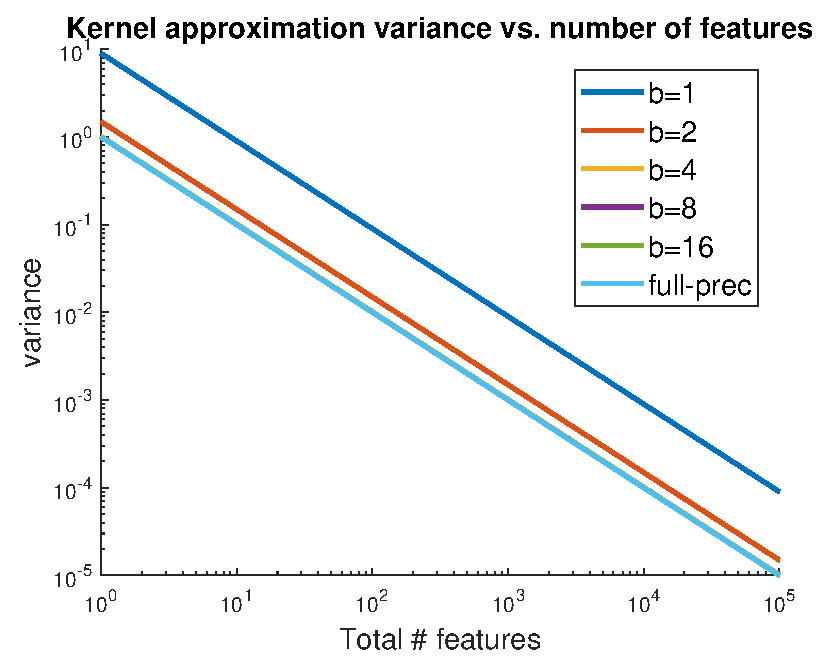
\includegraphics[width=0.4\textwidth]{figures/var_vs_numfeat.eps} &
		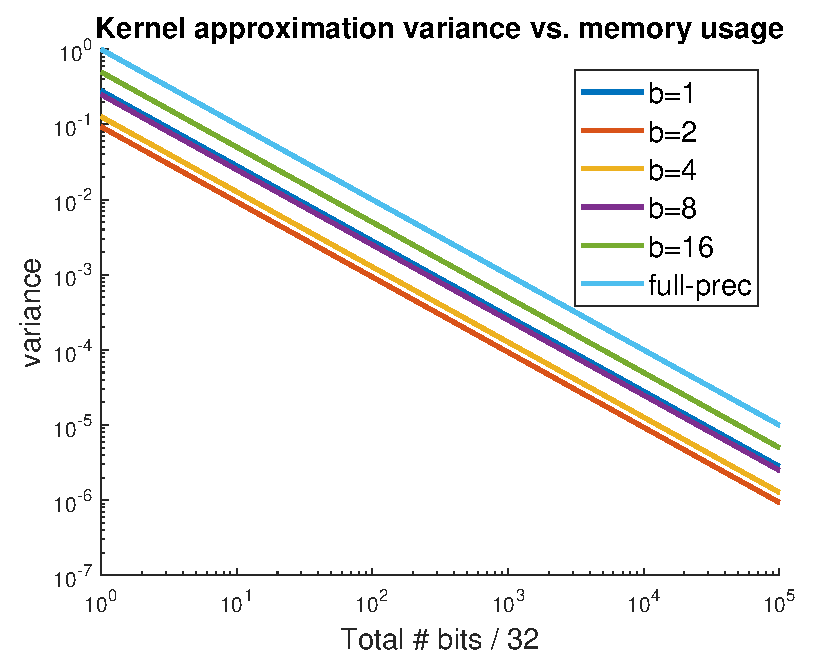
\includegraphics[width=0.4\textwidth]{figures/var_vs_numbits.eps}  \\
		(a) & (b) \\
	\end{tabular}
	\caption{Kernel Approximation Variance, as a function of the number of features used (a), and the amount of memory used (b).  Note that in the left plot, the 4-bit, 8-bit, 16-bit, and full-precision lines all overlap.}
\label{fig:kernel_approx_var}
\end{figure}

\subsection{Spectrum of Low-Precision RFF}
\label{sec:spectrum}
In this section, we analyze the effect that using low-precision has on the spectrum of the approximated kernel matrix.  We will be quantifying the size of the gap between the low-precision spectrum, and the full-precision spectrum.  We will now show that randomly quantizing an RFF matrix $Z$ with zero-mean noise ``elevates'' the spectrum of the quantized matrix (relative to the full precision matrix):
\begin{proposition}
	Let $Z$ be an $n$ by $d$ RFF matrix whose $i^{th}$ row is $z(x_i)$, and let $C$ denote the zero mean random quantization noise which is added to $Z$.  If $\lambda$ denotes the spectrum of $ZZ^T$, and $\tlambda$ denotes the spectrum of $(Z+C)(Z+C)^T$, it follows that $\expect{}{\sum_i \lambda_i} = n$, while $\expect{}{\sum_i \tlambda_i} \leq n + \frac{2n}{(2^b-1)^2}$.
\end{proposition}
\begin{proof}
	\begin{eqnarray*}
		\expect{}{\sum_i \lambda_i} &=& \expect{}{trace[ZZ^T]} \\
		&=& \expect{}{\sum_i z(x_i)^Tz(x_i)}\\
		&=& \sum_i k(x_i,x_i)\\
		&=& n \\
%		\expect{}{trace[ZZ^T]} &=& \expect{}{trace(USU^TUSU^T)}\\
%		&=& \expect{}{trace(US^2U^T)}\\
%		&=& \expect{}{\sum_i \lambda_i^2} \\
		\expect{}{\sum_i \lambda_i} &=& \expect{}{trace((Z+C)(Z+C)^T)} \\
		&=& 	\expect{}{trace(ZZ^T+CZ^T + ZC^T + CC^T)}  \\
		&=& \expect{}{trace(ZZ^T)} + \expect{}{trace(CC^T)} \\
		&=& n + \sum_i \expect{}{c_i^T c_i}, \;\;\text{where $c_i$ is the $i^{th}$ row of $C$}\\
		&=& n + \sum_{i=1}^n \sum_{j=1}^d \expect{}{c_{ij}^2} \\
		&\leq& n + nd\cdot \frac{2}{d(2^b-1)^2}\\
		&=& n + \frac{2n}{(2^b-1)^2}
	\end{eqnarray*}
	Above, we use the fact that $\expect{}{c_{ij}^2} \leq \frac{1}{4}\bigg(\frac{2\sqrt{2/d}}{2^b-1}\bigg)^2 = \frac{2}{d(2^b-1)^2}$.
\end{proof}

Notice that the spectrum $\tlambda$ of $(Z+C)(Z+C)^T$ relates to the spectrum $\tsigma$ of $(Z+C)$ via $\tlambda_i = \tsigma_i^2$.  Thus, letting $\sigma$ denote the spectrum of $Z$, we have shown that
$\expect{}{\sum_i \tsigma_i^2} > \sum_i \sigma_i^2$.  In other words, adding zero mean noise of any kind to a matrix elevates the $\ell_2$ norm of its spectrum.  This is intuitive because the noise will always increase the total weight on the diagonal of $ZZ^T$.

More interestingly, however, we can also show that if we take two random draws $C$ and $D$ of the quantization noise, the spectrum of $(Z+C)(Z+D)^T$ is also elevated relative to $ZZ^T$, even though the expected value of the entries of the diagonal of this matrix are \textit{equal} to the entries of the $ZZ^T$ diagonal.  This is because we can write $(Z+C)(Z+D)^T = ZZ^T + CZ^T + ZD^T + CD^T = ZZ^T + N$, where $N = CZ^T + ZD^T + CD^T$ is zero mean noise.  Thus, just like the spectrum of $Z+C$ was higher than that of $Z$ because we added zero mean noise $C$ to it, the spectrum of $(Z+C)(Z+D)^T$ will be higher than that of $ZZ^T$ because we are adding zero mean noise $N$ to it.  We show this in more detail in the proposition below:

\begin{proposition}
	Let $Z$ be an $n$ by $d$ RFF matrix whose $i^{th}$ row is $z(x_i)$, and let $C$, $D$ denote independent draws of zero mean random quantization noise of the same dimension as $Z$.  If $\lambda$ denotes the spectrum of $ZZ^T$, and $\tlambda$ denotes the spectrum of $(Z+C)(Z+D)^T$, it follows that 
	$\expect{}{\sum_i \lambda_i^2} = n + \frac{n^2-n}{d}$, while 
	$\expect{}{\sum_i \tlambda_i^2} \leq n + \frac{n^2-n}{d} +  \frac{4n^2}{d}\Big(\frac{1}{(2^b-1)^2} + \frac{1}{(2^b-1)^4}\Big)$.
\end{proposition}
\begin{proof}
Letting $A = ZZ^T$ and $\tA = (Z+C)(Z+D)^T$, we derive the following:
\begin{eqnarray*}
	\expect{}{\sum_i{\lambda_i^2}} &=& 	\expect{}{trace(A^T A)} \\
	&=& \expect{}{trace(ZZ^TZZ^T)}. \\
	\expect{}{\sum_i{\tlambda_i^2}} &=& \expect{}{trace(\tA^T\tA)} \\
	&=& \expect{}{trace((Z+D)(Z+C)^T(Z+C)(Z+D)^T)} \\
	&=& \expect{}{trace(ZZ^TZZ^T + ZC^TCZ^T + DZ^TZD^T + DC^TCD^T + \text{zero-mean})}\\ 
	&=& \expect{}{trace(ZZ^TZZ^T)} + \expect{}{trace(ZC^TCZ^T)} + \expect{}{trace(DZ^TZD^T)} + \expect{}{trace(DC^TCD^T)}\\
	&=& \expect{}{trace(ZZ^TZZ^T)} + \expect{}{trace(ZC^TCZ^T)} + \expect{}{trace(ZD^TDZ^T)} + \expect{}{trace(DC^TCD^T)}\\
	&=& \expect{}{trace(ZZ^TZZ^T)} + 2\expect{}{trace(ZC^TCZ^T)} + \expect{}{trace(DC^TCD^T)}.
\end{eqnarray*}
Now, we need to compute more precise values for the three terms in this expression.  For this purpose, we will repeatedly use the following fact, which applies to any matrices $A$, $B$ of equal dimensions:
$$trace[AB^TBA^T] = \sum_{i,j=1}^n \sum_{k,\hk=1}^d a_{jk}a_{j\hk}b_{ik}b_{i\hk}.$$
We will proceed one expression at a time:

\begin{itemize}
	\item Case 1: $A=B=Z$.
	\begin{eqnarray*}
		\expect{}{trace[ZZ^TZZ^T]} &=& \sum_{i,j=1}^n \sum_{k,\hk=1}^d \expect{}{z_{jk}z_{j\hk}z_{ik}z_{i\hk}}\\
		&=& \sum_{i=1}^n \sum_{k,\hk=1}^d \expect{}{z_{ik}^2}\expect{}{z_{i\hk}^2} + \sum_{i\neq j} \sum_{k=1}^d \expect{}{z_{jk}^2}\expect{}{z_{ik}^2}\\
		&=& \sum_{i=1}^n \sum_{k,\hk=1}^d \frac{1}{d^2} + \sum_{i\neq j} \sum_{k=1}^d \frac{1}{d^2}\\
		&=& nd^2\frac{1}{d^2} + (n^2-n)d\frac{1}{d^2}\\
		&=& n + \frac{n^2-n}{d}.
	\end{eqnarray*}
	Above, we used the fact that $\expect{}{z_{ik}^2} = \expect{w_k,b_k}{\frac{2}{d}\cos(w_k^T x_i + b_k)^2} = \frac{k(x_i,x_i)}{d} = \frac{1}{d}$.
	\item Case 2: $A=Z$, $B=C$.
	\begin{eqnarray*}
		\expect{}{trace[ZC^TCZ^T]} &=& \sum_{i,j=1}^n \sum_{k,\hk=1}^d \expect{}{z_{jk}z_{j\hk}c_{ik}c_{i\hk}}\\	
		&=& \sum_{i,j=1}^n \sum_{k=1}^d \expect{}{z_{jk}^2}\expect{}{c_{ik}^2}\\	
		&\leq& \sum_{i,j=1}^n \sum_{k=1}^d \frac{1}{d}\cdot \frac{2}{d(2^b-1)^2}\\	
		&=& n^2d \cdot \frac{1}{d}\cdot \frac{2}{d(2^b-1)^2}\\	
		&=& \frac{2n^2}{d(2^b-1)^2}.
	\end{eqnarray*}
	Above, we used the fact that $\expect{}{c_{ik}^2} \leq \frac{1}{4}\bigg(\frac{2\sqrt{2/d}}{2^b-1}\bigg)^2 = \frac{2}{d(2^b-1)^2}$, and that $\expect{}{z_{ik}^2} = \frac{1}{d}$.
	\item Case 3: $A=C$, $B=D$.
	\begin{eqnarray*}
		\expect{}{trace[CD^TDC^T]} &=& \sum_{i,j=1}^n \sum_{k,\hk=1}^d \expect{}{c_{jk}c_{j\hk}d_{ik}d_{i\hk}}\\
		&=& \sum_{i,j=1}^n \sum_{k=1}^d \expect{}{c_{jk}^2}\expect{}{d_{ik}^2}\\
		&\leq& \sum_{i,j=1}^n \sum_{k=1}^d \bigg(\frac{2}{d(2^b-1)^2}\bigg)^2\\
		&=& n^2d \cdot\frac{4}{d^2(2^b-1)^4}\\
		&=& \frac{4n^2}{d(2^b-1)^4}.
	\end{eqnarray*}
\end{itemize}
Combining these three results concludes the proof of the proposition.
\end{proof}

In Figures \ref{fig:spectrums} and \ref{fig:indep_quant} in Section \ref{sec:experiments} we validate these results empirically. We observe that the spectra of our kernel approximation matrices are much higher than the actual spectrum of the exact kernel matrix, in the case where we use 1, 2, or 4 bits to quantize our features.  We also observe that using $(Z+C)(Z+D)^T$ instead of $(Z+C)(Z+C)^T$ gives a smaller increase to the spectrum.

\section{Generalization Performance of Low-Precision RFF}
\label{sec:gen}

\begin{theorem} (extending Theorem 1 of $[4]$ to LP-RFF): \\
\label{thm:gen}
Let $\phi:\cX\times\Omega\rightarrow\RR$ be a set of feature functions such that $\sup_{x,w}|\phi(x;w)| \leq 1$. Assume there exists a family of deterministic quantization functions $\{Q_{\theta}:\RR\rightarrow\RR \;|\; \theta\in\Theta \}$, parameterized by some parameter $\theta\in\Theta$.  Let $p_{\Theta}$ be a probability distribution over $\Theta$, $p_{\Omega}$ be a probability distribution over $\Omega$, and define $p(w,\theta) = p_{\Omega}(w)p_{\Theta}(\theta)$.
Define the quantized feature functions as $\phi'(x;w,\theta) = Q_{\theta}(\phi(x;w))$, and define
$$\cF_p = \bigg\{f(x) = \int_{\Omega\times\Theta} \alpha(w,\theta) \phi'(x;w,\theta)dwd\theta \;\;\bigg|\;\; |\alpha(w,\theta)| \leq Cp(w,\theta)\bigg\}.$$
Suppose the cost function $c(y,y') = c(yy')$, with $c(yy')$ $L$-Lipschitz.  Then for any $\delta > 0$, if the training data $\{x_i,y_i\}_{i=1}^n$ are drawn iid from some distribution $P$, Algorithm \ref{alg:lprff}  returns a function $\hat{f}$ that satisfies:
$$R[\hat{f}] - \min_{f\in\cF_p}R[f] \leq O\Bigg(\bigg(\frac{1}{\sqrt{n}} + \frac{1}{\sqrt{m}}\bigg)LC \sqrt{\log\frac{1}{\delta}}\Bigg)$$
with probability at least $1-2\delta$ over the training dataset and the choice of the parameters $w_i,\theta_i$.
(Here, $R[F] = \expect{(x,y)\sim P}{c(f(x),y)}$)
%with the property that $\expect{\theta}{Q_{\theta}(z)} = z$, where this expectation is taken with respect to some probability distribution over $\theta$.
\end{theorem}

\begin{algorithm}
\caption{%
	Low-Precision Weighted Sum of Random Kitchen Sinks Training (adapted from $[4]$)%
}
\label{alg:lprff}
\begin{algorithmic}[1]
	\renewcommand{\algorithmicrequire}{\textbf{Input}}
	\REQUIRE
	A dataset $\{x_i,y_i\}_{i=1}^n$ of $n$ points, a family of bounded feature functions $|\phi(x;w)|\leq 1$ parameterized by $w\in\Omega$, a family of bounded quantization functions $|Q(z;\theta)| \leq 1$ parameterized by $\theta \in \Theta$, an integer $m$, a scalar $C$, probability distributions  $p_{\Omega}$ and $p_{\Theta}$ over $\Omega$ and $\Theta$.
	\renewcommand{\algorithmicrequire}{\textbf{Output}}
	\REQUIRE
	A function $\hat{f}(x) = \sum_{i=1}^m Q(\phi(x;w_i);\theta_i) \alpha^*_i$.
	\STATE Draw $w_1,\ldots,w_m$ from $p_{\Omega}$, and $\theta_1,\ldots,\theta_m$ from $p_{\Theta}$.
	\STATE Featurize the input: $z_i \leftarrow [Q(\phi(x_i;w_1);\theta_1),\ldots,Q(\phi(x_i;w_m);\theta_m)]^T$.
	\STATE With the $w_i$ and $\theta_i$ fixed, solve the empirical risk minimization problem:
	\begin{eqnarray*}
		\alpha* =\argmin_{\alpha\in\RR^m} \frac{1}{n}\sum_{i=1}^n c(\alpha^T z_i,y_i)\\
		s.t. \|\alpha\|_\infty < C/m
	\end{eqnarray*}
	\RETURN $\hat{f}(x) = \sum_{i=1}^m Q(\phi(x;w_i);\theta_i) \alpha^*_i$.
\end{algorithmic}
\end{algorithm}


\noindent \textbf{Open Question}: How does the family of functions $\cF_p$ defined in Proposition 3 compare to the one in $[4]$ (Rahimi and Recht, 2008)?	

\subsection{``Deterministic'' Quantization Functions}
\label{sec:deterministic}
In Theorem \ref{thm:gen}, we defined a set of deterministic quantization functions
$\{Q_{\theta}:\RR\rightarrow\RR \;|\; \theta\in\Theta \}$, parameterized by some parameter $\theta\in\Theta$.
We now discuss how to construct these.  The idea is simple: For every quantization interval $[a,c]$, we choose a threshold value $t \in [a,c]$ uniformly at random.  Then if a certain unquantized feature $z$ falls in this interval, we will set $Q_t(z)= a$ if $z \leq t$, and $Q_t(z) = c$ if $z > t$.  It is easy to show that $\expect{t}{Q_t(z)} = z$:
\begin{eqnarray*}
	\expect{t}{Q_t(z)} &=& a \cdot \Prob[z \leq t] + c \cdot \Prob[z > t]  \\
	&=& a \cdot \frac{c-z}{c-a} + c\cdot \frac{z-a}{c-a} \\
	&=& \frac{ac - az + cz - ac}{c-a} \\
	&=& z.
\end{eqnarray*}
Thus, if for every quantization interval we draw a random threshold $t_i$ as described, and concatenate these thresholds as $\theta = (t_1,\ldots,t_{2^b-1})$, we have successfully constructed a set of unbiased and deterministic quantization functions, as desired.

\subsection{Effect of quantization noise at test time}
\label{sec:reduce_test_noise_theory}
In this section, we show that the quantization noise at test time results in larger expected 
mean-squared error, in the context of kernel ridge regression.

\begin{theorem}
\label{thm:testvar}
Let $Q:\RR^m\rightarrow\RR^m$ be an unbiased (element-wise) random quantization function with bounded variance ($\var{}{Q(z)_i} \leq \tsigma^2 \; \forall z,i$), and let $f_w(z) = w^T z$ be a fixed regression model.  It follows that the expected mean-squared error, using quantized features $Q(z(x))$, satisfies $$\expect{}{\Big(f_w(Q(z(x))) - y\Big)^2} \leq \expect{}{\Big(f_w(z(x)) - y\Big)^2} + \|w\|^2\tsigma^2.$$
\end{theorem}

\begin{proof}
Let $z(x)$ denote the full precision RFF representation for $x$, and $Q(z(x)) = z(x) + \eps_x$ represents the randomly quantized representation.
\begin{eqnarray*}
	\expect{}{\Big(f_w(Q(z(x))) - y\Big)^2} &=& \expect{}{(w^T (z(x) + \eps_x) -y)^2} \\
	&=& \expect{}{(w^T z(x) + w^T \eps_x -y)^2} \\
	&=& \expect{}{(w^T z(x) - y)^2)} + \expect{}{(w^T \eps_x)^2} \\
	&=&  \expect{}{\Big(f_w(z(x)) - y\Big)^2} + \expect{}{\Big(\sum_i w_i \eps_{x,i}\Big)^2} \\
	&=&  \expect{}{\Big(f_w(z(x)) - y\Big)^2}+ \sum_i w_i^2 \expect{}{\eps_{x,i}^2} \\
	&=&  \expect{}{\Big(f_w(z(x)) - y\Big)^2}  + \|w\|^2\expect{}{\eps_{x,1}^2} \\
	&\leq&  \expect{}{\Big(f_w(z(x)) - y\Big)^2} + \|w\|^2\tsigma^2.
\end{eqnarray*}
\end{proof}
This theorem shows that our expected error on a test point $(x,y)$, if we use quantized features at test time, is in expectation $\|w\|^2\tsigma^2$ larger than the expected error if we used the full precision features at test time.  In the case where $Q$ quantizes each feature into $b$ bits, $\tsigma^2= \frac{2}{m(2^b-1)^2}$.
This suggests that it could be desirable, in certain contexts, to train using low precision (to speed up training), but use full precision features at test time.

\subsection{Fixed Design Kernel Ridge Regression}
\label{sec:fixed_design}
In this section, we will show, in the context of ``fixed design'' linear regression, that the generalization performance of the model depends deeply on the spectrum of the kernel matrix (or kernel approximation matrix) used to train the model.

``Fixed design'' linear regression is a particularly straightforward to analyze form of linear regression, in which the test points are the same as the training points; importantly, however, the training labels $y_i$, and test labels $y_i'$, are noisy, corresponding to zero-mean noise added to the unobserved ``true labels'' $y_i^*$. The noise values added to the labels are assumed to be uncorrelated with common variance $\sigma^2 > 0$.  In the case of kernel ridge regression, the learned classifier predicts regression values of $\hy = K(K+\lambda\id)^{-1}y = Ay$ on the training set, for $A=K(K+\lambda\id)^{-1}$.  Letting $K=U\Sigma U^T$, where $\sigma_i$ is the $i^{th}$ largest eigenvalue of $K$, and $U_i$ is the corresponding eigenvector, we have that $A = U\Gamma U^T$, with $\gamma_i = \frac{\sigma_i}{\sigma_i + \lambda}$.

In his course notes for Advanced Methods for Data Analysis [6], Ryan Tibshirani shows that the expected test error can be precisely calculated as a function of the training error, the variance $\sigma^2$ of the label noise, and the ``degrees of freedom'' of the classifier (which corresponds to the trace of $A$, when the classifier predicts $\hy = Ay$ on the training set).  The precise relation is as follows:

\begin{eqnarray*}
	\expect{}{\frac{1}{n}\sum_{i=1}^n (\hy_i - y_i')^2} &=& \expect{}{\frac{1}{n}\sum_{i=1}^n (\hy_i - y_i)^2} + \frac{2\sigma^2}{n}df(\hy)\\
\end{eqnarray*}

We now show that in the context of kernel ridge regression, the right hand side of this expression can be simplified to only depend on the eigenvalues and eigenvectors of $K$.

\begin{proposition}
	Letting $A=K(K+\lambda\id)^{-1}$, where $K=U\Sigma U^T$ is a kernel matrix with eigenvectors $U_i$ and eigenvalues $\sigma_i$, it holds that the expected test error in the context of fixed design linear regression can be expressed as follows:
\begin{eqnarray*}
	\expect{\epsilon,\epsilon'}{\frac{1}{n}\|A(y^*+\eps) - (y^*+\eps')\|^2} 
	&=& \frac{1}{n}\sum_{i=1}^n \bigg(\frac{\sigma_i}{\sigma_i + \lambda}-1\bigg)^2 (U_i^T y^*)^2 + \frac{\sigma^2}{n}\sum_{i=1}^n \bigg(\frac{\sigma_i}{\sigma_i + \lambda}\bigg)^2 + \sigma^2,
\end{eqnarray*}	
\end{proposition}
\begin{proof}
We simplify the expression from Ryan Tibshirani's course notes, using the facts that $\hy = A(y^* + \eps)$, $y' = y + \eps'$, $A = U\Gamma U^T$ with $\gamma_i = \frac{\sigma_i}{\sigma_i + \lambda}$, and $df(\hy) = trace(A) = \sum_i \gamma_i = \sum_i \frac{\sigma_i}{\sigma_i + \lambda}$.

\begin{eqnarray*}
	\expect{\epsilon,\epsilon'}{\frac{1}{n}\|A(y^*+\eps) - (y^*+\eps')\|^2} 
	&=& \expect{\epsilon}{\frac{1}{n}\|A(y^*+\eps) - (y^*+\eps)\|^2} + \frac{2\sigma^2}{n}df(\hy) \\
	&=& \frac{1}{n}\expect{\epsilon}{\|(A-\id)(y^*+\eps)\|^2} + \frac{2\sigma^2}{n}Tr(A) \\
	&=& \frac{1}{n}\expect{\epsilon}{\|U(\Gamma-\id)U^T(y^*+\eps)\|^2} + \frac{2\sigma^2}{n}Tr(A) \\
	&=& \frac{1}{n}\expect{\epsilon}{(y^*+\eps)^TU(\Gamma-\id)U^TU(\Gamma-\id)U^T(y^*+\eps)} + \frac{2\sigma^2}{n}Tr(A) \\
	&=& \frac{1}{n}\expect{\epsilon}{Tr\bigg((y^*+\eps)^TU(\Gamma-\id)^2 U^T(y^*+\eps)\bigg)} + \frac{2\sigma^2}{n}Tr(A) \\
	&=& \frac{1}{n}\expect{\epsilon}{Tr\bigg(U(\Gamma-\id)^2 U^T(y^*+\eps)(y^*+\eps)^T\bigg)} + \frac{2\sigma^2}{n}Tr(A) \\
	&=& \frac{1}{n}\expect{\epsilon}{Tr\bigg(U(\Gamma-\id)^2 U^T(y^* y^{*T} + \eps y^{*T} + y^*\eps^T + \eps \eps^T\bigg)} + \frac{2\sigma^2}{n}Tr(A) \\
	&=& \frac{1}{n}Tr\bigg(U(\Gamma-\id)^2 U^T\Big(y^* y^{*T} + \expect{\epsilon}{ \eps \eps^T}\Big)\bigg) + \frac{2\sigma^2}{n}Tr(A) \\
	&=& \frac{1}{n}Tr\bigg(U(\Gamma-\id)^2 U^T\Big(y^* y^{*T} + \sigma^2 \id \Big)\bigg) + \frac{2\sigma^2}{n}Tr(A) \\
	&=& \frac{1}{n}Tr\bigg((\Gamma-\id)^2 U^T y^* (U^T y^*)^T\bigg)  + \frac{\sigma^2}{n}Tr\bigg((\Gamma-\id)^2\bigg) + \frac{2\sigma^2}{n}Tr(U\Gamma U^T) \\
	&=& \frac{1}{n}\sum_{i=1}^n (\gamma_i-1)^2 (U_i^T y^*)^2 + \frac{\sigma^2}{n}\sum_{i=1}^n (\gamma_i-1)^2 + \frac{2\sigma^2}{n}\sum_{i=1}^n \gamma_i\\
	&=& \frac{1}{n}\sum_{i=1}^n (\gamma_i-1)^2 (U_i^T y^*)^2 + \frac{\sigma^2}{n}\sum_{i=1}^n \Big(\gamma_i^2 -2\gamma_i + 1 + 2\gamma_i\Big) \\
	&=& \frac{1}{n}\sum_{i=1}^n (\gamma_i-1)^2 (U_i^T y^*)^2 + \frac{\sigma^2}{n}\sum_{i=1}^n \gamma_i^2 + \sigma^2
\end{eqnarray*}
\end{proof}

This result shows the fundamental relationship between the spectrum of the kernel matrix, and the generalization performance of the regression model.
\section{Training a model using low-precision random features}
\label{sec:train}
In this section, we present several possible ways of training a model on top of low-precision random Fourier features.  Importantly, any of the options outlined below which uses low-precision for both train/test would be inherently limited in terms of how close to the global optimum they could get, as discussed in the recent High-Accuracy Low-Precision Training paper $[7]$.  Perhaps, however, the error introduced by this quantization could be more than made-up for by the ability to learn a model in a higher-dimensional, more expressive, feature space.

\begin{itemize}
\item \textbf{LM-HALM}: `LM-HALP'' is the version of HALP designed for learning linear models, presented as Algorithm 4 in $[7]$. One potential down-side to this approach is that it would mean that the learned model would be full-precision, which may or may not be desirable (for example, computing the full-precision gradient over the entire dataset could be prohibitively expensive, and perhaps even impossible in the case where the full-precision model wouldn't fit in memory).
\item \textbf{Perceptron updates}: We could use the perceptron algorithm for model updates, 
which would ensure that all operations could be done in integer arithmetic.
\item\textbf{Quantized SGD updates (``LP-SGD'')}: Consider the full-precision SGD update of
the form $w_{t+1} = w_t + g_t z_t$, where $z_t = z(x_t) \in \RR^m$ is the random
feature representation corresponding to the randomly chosen training point $x_t$ at
time $t$.  We could replace this update by updates of the form 
$w_{t+1} = w_t + \tg_t \tz_t$, where $\expect{}{\tg_t} = g_t$, and $\tg_t$ is stored in
low-precision format.  For example, in the case of logistic regression, 
$g_t = \eta \big(y_t - p_t\big)$, where $y_t\in\{0,1\}$ is the label for $x_t$, $\eta \in \RR$ is the learning
rate, and $p_t = p(Y_t=1|z_t,w_t) = (1+\exp(-w_t^Tz_t))^{-1}$. 
If $\tg_t$ is in $(\delta,b)$ low-precision format, and $\tz_t$ is in
$(\delta',b')$ format, then $w_t$ would be in $(\delta\delta',b+b')$ format.
\item \textbf{LP-SVRG}: We could directly use LP-SVRG.
\item \textbf{Update dual variables instead of primal}: In terms of the dual variables $\alpha_i$, the
model becomes $f(x) = \sum_{i=1}^n \alpha_i z(x_i)^T z(x)$. Letting 
$Z\in \RR^{n\times m}$ be the matrix whose $i^{th}$ row is $z(x_i)$, this can be
rewritten as $\alpha^T (Z z(x))$.  If the random features are binary, $Zz(x)$ 
can be implemented very efficiently, and its output is an integer vector (note that for huge $Z$,
this operation can be distributed across a cluster of machines).
If $\alpha$ is stored in low-precision format (as it would be if updates of the form described above
for perceptron or LP-SGD are used), this dot-product could be performed using low-precision
integer arithmetic, which can also be implemented fast.  As far as updating the values of
the dual parameters $\alpha_i$ during training, we can simply simulate the primal updates of the form 
$w_{t+1} = w_t + \tg_t z_t$ by using $\alpha_t = \alpha_t + \tg_t$, where here I am using 
$\alpha_t$ to denote the dual parameter corresponding to the random point $x_t$ chosen at time $t$.
\item \textbf{Distributed optimization}: We could also consider large-scale distribution optimization algorithms (\eg, $[1,2]$) in order to speed up training.
\end{itemize}


\subsection{Computing the low-precision random features}
In this entire document so far, we have considered the setting where we compute quantized features by first computing the full precision features, and then performing random quantization.  Another option is to 
first quantize $x$, $W$, and $b$, as $\tx$, $\tW$, $\tb$.  Then, compute $\cos(\tW^T \tx + \tb)$, and quantize the output.
One important thing to note is that quantizing $x$,$W$, and $b$ in such a way that $\expect{\tx,\tW,\tb}{\tW^T\tx + \tb} = W^Tx+b$ does \textit{not} mean that $\expect{\tx,\tW,\tb}{\cos(\tW^T\tx + \tb)} = \cos(W^Tx + b)$.  Thus, features generated in this way would not necessarily produce unbiased estimates of the kernel function, which satisfy $\expect{}{z(x)^Tz(y)} = k(x,y)$.

\noindent \textbf{Open Question}: Is there anything we can prove about computing low-precision features in the above manner? Would they perform well empirically?

\section{Experiments}
\label{sec:experiments}
\subsection{Kernel Ridge Regression}
\begin{figure}
\centering
\begin{tabular}{c c}
	\includegraphics[width=.45\linewidth]{figures/kernel_approx_error.pdf} &
	\includegraphics[width=.45\linewidth]{figures/kernel_approx_error_n_fp.pdf} \\
	(a) & (b) \\
	\includegraphics[width=.45\linewidth]{figures/valid_l2.pdf} &
	\includegraphics[width=.45\linewidth]{figures/valid_l2_n_fp.pdf}  \\
		(c) & (d) \\
\end{tabular}
\caption{Kernel approximation and validation L2 loss for Kernel Ridge Regression on UCI Census dataset. (a) and (b) compare different precision representation under same memory bits budgets. (c) and (d) compare different precision representation with the same number of random Fourier features.}
\label{fig:kernel_and_l2}
\end{figure}

We use UCI Census dataset for the experiments on kernel ridge regression. This dataset contains 16k training samples with 119 original features. Besides from reporting the kernel approximation errors, we also report the validation l2 loss in the regression problem. The reported l2 loss for each feature precision is from a grid search over $\{1e^{-6}, 1e^{-5}, ..., 1e^{-1}, 1, 10, 100\}$. To report statistically meaningful results, we average the performance metrics from 5 stochastic quantization using different random seeds. We uniformly use Gaussian kernels with $\sigma=30.0$ for our experiments on kernel ridge regression.

\paragraph{Kernel approximation error and validation l2 loss}
As shown in Figure~\ref{fig:kernel_and_l2} (b) and (d), when using the same number of random Fourier features, the kernel approximation error and validation l2 loss only start to observably degrade after the the precision gets lower than 8 bits. For precision using 8 bits or higher number of bits, the validation l2 loss closely overlap with the ones from full precision random Fourier features. Further more, we compare the performance of feature representation in different precision under the same memory bits budget for each data sample. Kernel methods based on RFF typically improves when more RFF presents, while more precise feature representation can demonstrate lower approximation error. \emph{Indeed, under the memory budgets, we observe a trade-off between the number of RFF and the representation precision of RFF in~\ref{fig:kernel_and_l2}(a) and (b). Specifically, under different memory budget for the RFF representation of each data sample, 2 or 4 bits representation presents the best kernel approximation, while 8 bits demonstrates the best validation l2 loss consistently.}


\begin{figure}
	\centering
	\begin{tabular}{c c}
		\includegraphics[width=.45\linewidth]{figures/spectrum_1024.pdf} &
		\includegraphics[width=.45\linewidth]{figures/spectrum_8192.pdf}  \\
		(a) & (b) \\
		\includegraphics[width=.45\linewidth]{figures/different_spectrum_with_same_kernel_approx_error_log.pdf} &
		\includegraphics[width=.45\linewidth]{figures/different_spectrum_with_same_kernel_approx_error.pdf}\\
		(c) & (d)
	\end{tabular}
	\caption{Spectrum (eigen values) of the kernel matrix. The spectrums from different precision representation are shown under a) 3.2k (equivalent to 1024 full precision rffs) and b) 25.6k bits memory budget (equivalent to 8192 full precision rffs) for the feature of each sample. (c) Configurations with similar approximation errors can demonstrate very different spectrum; we compare the 1 bit representation to the full precision configurations giving 1) the highest approx. error that is lower than the 1 bit configuration 2) the lowest approx. error that is higher than the 1bit configuration. (c) Replot (b) in decimal scale to visualize the difference of spectrums; the spectrums from kernel matrix using 1) a single stochastic quantization and 2) two independent stochastic quantization for the feature matrix and its transpose. \emph{Note in (c) and (d), we can observe independent quantization for RFF matrix and its transpose (indep. noise curves in the figures) presents spectrum closer to the exact kernel than using the same stochastic quantization for RFF matrix and its transpose.} }
	\label{fig:spectrums}
\end{figure}

\paragraph{Spectrum of kernel matrix correlates with l2 loss}
In our theory in Section~\ref{}, we have been discussing how low precision introduce quantization variance, which results in bumping up the spectrum of kernel matrix. In Figure~\ref{fig:spectrums} (a), we demonstrate the kernel matrix spectrum from 8192 random Fourier features in different precision. 
In Figure~\ref{fig:spectrums} (a), we can observe 8, 16 and 32 bits representation has spectrums close to the spectrum of full precision RFF kernel matrix. However, for 4, 2 and 1 bits representation has significantly higher spectrums than 8, 16 and 32 bits representation. Remember that in Figure~\ref{fig:kernel_and_l2}, we have seen 8, 16 and 32 bits representation demonstrates similar l2 loss, while 4, 2 and 1 bits can show observably worse performance. Thus we believe 

\begin{figure}
	\centering
	\begin{tabular}{c c}
		\includegraphics[width=.45\linewidth]{figures/valid_l2_var_reduction.pdf} &
		\includegraphics[width=.45\linewidth]{figures/valid_l2_n_fp_var_reduction.pdf} \\
		(a) & (b)
	\end{tabular}
	\caption{We train with low precision rffs and test with full precision rffs. Though the model is trained with low precision features, the test l2 loss can be improved by reducing variance in test rffs. (a) compare different precision representation under same memory bits budgets. (b) compare different precision representation with the same number of random Fourier features.}
	\label{fig:var_reduction}
\end{figure}


\begin{figure}
	\centering
	\begin{tabular}{c c}
		\includegraphics[width=.45\linewidth]{figures/spectrum_1024_indep.pdf} &
		\includegraphics[width=.45\linewidth]{figures/spectrum_8192_indep.pdf} \\
		(a) & (b) \\
		\includegraphics[width=.45\linewidth]{figures/spectrum_1024_indep_log.pdf} &
		\includegraphics[width=.45\linewidth]{figures/spectrum_8192_indep_log.pdf} \\
		(c) & (d)
	\end{tabular}
	\caption{Spectrum (eigen values) of the kernel matrix. (a) The spectrum from different precision representation under 3.2k bits memory budget (1024 full precision rffs) for the feature of each sample. (b) The spectrum from different precision representation under 25.6k bits memory budget (1024 full precision rffs) for the feature of each sample.}
\end{figure}

%
%512 2 bits, 4096 fp 8192 fp, 4096 1 bit



\section{Future Directions}
\label{sec:future}
The next directions we plan to explore are as follows:
\begin{enumerate}
\item \textbf{Variable Precision}:  Storing the higher variance directions in the RFF feature space with more bits.  We also want to think more deeply about how to integrate the matrix factorization results into the kernel approximation context, perhaps in the context of the Nystrom method.
\item \textbf{Deterministic Rounding}: Testing the deterministic rounding ideas from Section \ref{sec:deterministic} empirically.
\item \textbf{Fixed Design Linear Regression}: Running controlled experiments in the fixed design context, to more precisely understand the effect the different approximate spectra are having on generalization performance.
\item \textbf{Training with LP-RFF}: Developing theoretically sound and fast algorithms for training using low-precision features.
\end{enumerate}
%(z_x+\teps_x)(z_y+\teps_y)$, where $\teps_x \sim X_{z_x}^{-\sq,\sq}$, and $\teps_y \sim X_{z_y}^{-\sq,\sq}$.
%Then $\var{}{\tS} = 4 - z_x^2 z_y^2$.
\section{References}
\noindent$[1]$ Large Scale Kernel Learning using Block Coordinate Descent.
Stephen Tu, Rebecca Roelofs, Shivaram Venkataraman, Benjamin Recht. \url{https://arxiv.org/pdf/1602.05310.pdf}. \\
$[2]$ CoCoA: A General Framework for Communication-Efficient Distributed Optimization.
Virginia Smith, Simone Forte, Chenxin Ma, Martin Takac, Michael I. Jordan, Martin Jaggi.  \url{https://arxiv.org/abs/1611.02189} \\
$[3]$ On the Error of Random Fourier Features. Dougal J. Sutherland, Jeff Schneider. UAI 2015. \url{https://arxiv.org/abs/1506.02785}\\
$[4]$ Weighted Sums of Random Kitchen Sinks: Replacing minimization with randomization in learning. Ali Rahimi, Ben Recht. NIPS 2008.\\
$[5]$	Random Features for Large-Scale Kernel Machines. Ali Rahimi, Benjamin Recht. NIPS 2007.\\
$[6]$  Course Notes: Advanced Methods for Data Analysis, Carnegie Mellon University.  Ryan Tibshirani, Spring 2014. \url{http://www.stat.cmu.edu/~ryantibs/advmethods/notes/df.pdf}\\
$[7]$ High-Accuracy Low-Precision Training. Christopher De Sa, Megan Leszczynski, Jian Zhang, Alana Marzoev,
Christopher Aberger, Kunle Olukotun, Christopher Re. \url{https://arxiv.org/pdf/1803.03383.pdf}
\end{document}
